\chapter{Benchmarks}

In this chapter, we measure the performance of our implementation. We quantify the impact of different input size and algorithm parameters. In the end, we compare our implementation with an original python implementation of the algorithm.

All the data was measured using an NVIDIA RTX 3080 graphics card with Intel i5 6600K processor. We used an M.2 SSD disk.

\todo{methodology? Each value presented in this chapter is a mean of several runs of the algorithm. }

\section{Relative performance of individual parts}

\begin{figure}
	\centering
	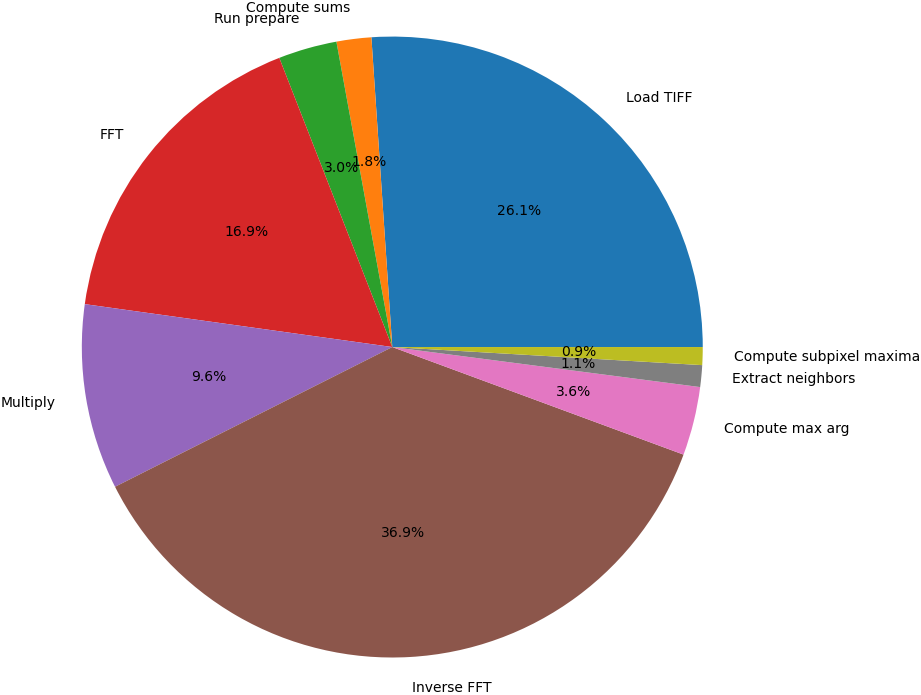
\includegraphics[width=0.7\textwidth]{img/eval/individual-parts}
	\caption{Relative performance of individual parts of the algorithm. The data was measured from a run of the algorithm with a configuration of 90 subregions with size $120 \times 120$. The size of the neigborhood was set to maximal value 9. }
	\label{individual-parts}
\end{figure}

We begin with an overview of all the kernels used in the implementation. \Cref{individual-parts} shows how much time the implementation spends in individual kernels. We can see, that the most demanding parts are loading of the TIFF and the cross--correlation, which is computed using the multiply kernel and the Fourier transforms.

The figure is mentioned here only to get general idea about the performance. It captures relative performance of the kernels for 90 subregions with size $120 \times 120$, which is roughly in the middle of the range of expected values. Different parts depend on different parameters, so for some other input size, the relative performance would look dissimilar. The load TIFF subroutine depends only on the size of the TIFF, while the rest of the algorithm depends on the number of subregion. So, for instance, it is possible to find a configuration that makes load TIFF the longest part. 

\section{Cross--correlation}
First, we measure the performance of cross--correlation when computed using Fourier transform. We show the dependence between running time and size and number of subregions. Since the cross--correlation is computed using three parts, we analyze them one by one.


\subsection{Fourier transforms}
\begin{figure}
	\centering
	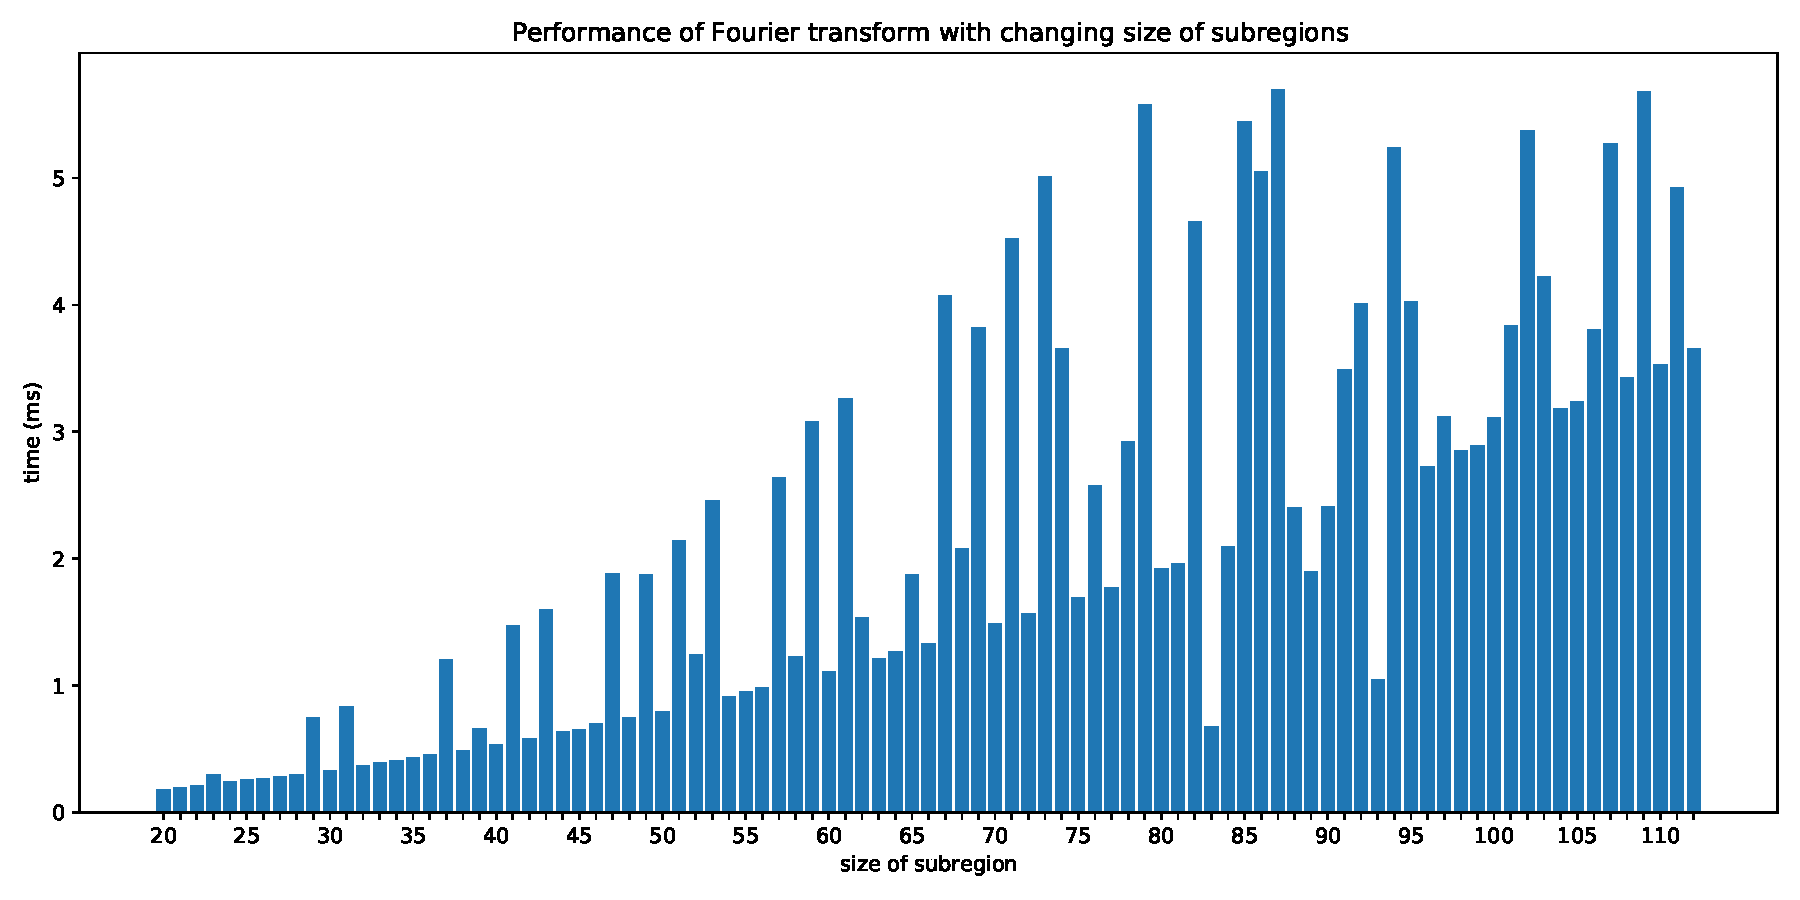
\includegraphics[width=\textwidth]{img/eval/Fourier-transform-size}
	\caption{Performance of Fourier transform with changing size of subregions. It was measured from a run of the algorithm with a configuration of 110 subregions. The size on the x axis denotes half of length of one side of subregion.}
	\label{Fourier-transform-size}
\end{figure}

In the \cref{Fourier-transform-size}, we can see how the forward Fourier transform executed by the cuFFT library depends on the size of subregions. We can see that the computation time increases with the size of the subregions, following the $\mathcal{O}(n \log n)$ time complexity of FFT. However, there are quite a few outliers --- sizes, for which the function does not perform very well. That can be explained by the following sentence cited from the cuFFT documentation: ``Algorithms highly optimized for input sizes that can be written in the form $2^a3^b5^c7^d$''. It means that all sizes, whose factorization contains a prime greater than 7 perform poorly. Choosing a bigger size with nice factorization results in better performance.

We can also see, that sizes 83 and 93 perform surprisingly well. We have measured it consistently. The reason behind such behavior is probably specific for cuFFT implementation.

The dependence of inverse Fourier transform on size of subregions looks very similar to the \cref{Fourier-transform-size} for the same reasons.

(Do jedneho grafu vsetky velkosti )

\section{Load TIFF}



\section{Float versus double}




\section{Speedup compared to original python implementation}


\section{Memory consumption}


overall performance - compare with python

batch size for different subregion sizes and count

different subregion sizes and count

sum - compare N to size of one slice, to batch size, to number of slices - how?